\documentclass{tufte-handout}

%\geometry{showframe}% for debugging purposes -- displays the margins

\usepackage{amsmath}

% Set up the images/graphics package
\usepackage{graphicx}
\setkeys{Gin}{width=\linewidth,totalheight=\textheight,keepaspectratio}
\graphicspath{{graphics/}}

\title{Carbohydrate Digestion and Absorption}
\author{Olivia Anderson and Dave Bridges}
\date{}  % if the \date{} command is left out, the current date will be used

% The following package makes prettier tables.  We're all about the bling!
\usepackage{booktabs}

% The units package provides nice, non-stacked fractions and better spacing
% for units.
\usepackage{units}

% The fancyvrb package lets us customize the formatting of verbatim
% environments.  We use a slightly smaller font.
\usepackage{fancyvrb}
\fvset{fontsize=\normalsize}

% Small sections of multiple columns
\usepackage{multicol}

% Provides paragraphs of dummy text
\usepackage{lipsum}

% These commands are used to pretty-print LaTeX commands
\newcommand{\doccmd}[1]{\texttt{\textbackslash#1}}% command name -- adds backslash automatically
\newcommand{\docopt}[1]{\ensuremath{\langle}\textrm{\textit{#1}}\ensuremath{\rangle}}% optional command argument
\newcommand{\docarg}[1]{\textrm{\textit{#1}}}% (required) command argument
\newenvironment{docspec}{\begin{quote}\noindent}{\end{quote}}% command specification environment
\newcommand{\docenv}[1]{\textsf{#1}}% environment name
\newcommand{\docpkg}[1]{\texttt{#1}}% package name
\newcommand{\doccls}[1]{\texttt{#1}}% document class name
\newcommand{\docclsopt}[1]{\texttt{#1}}% document class option name

\begin{document}
\maketitle% this prints the handout title, author, and date

\begin{abstract}
The majority of caloric intake worldwide is carbohydrates, with most people eating about half of their total calories in this form.  There is a lot of variation in how we digest and absorb different carbohydrates and this in turn plays a major role in how blood glucose is controlled.  In this lecture we will discuss the digestive processes specific to carbohydrates starting in the oral cavity all the way to the end of the tract. We will go over absorption and transportation of simple carbohydrates through the enterocyte to circulation.
\end{abstract}

\tableofcontents


\pagebreak


\section{Learning Objectives}

\begin{itemize}
\item Describe digestion of carbohydrates starting in the oral cavity
\item Apply knowledge of carbohydrate structure to carbohydrate- specific digestive enzymatic properties
\item Understand absorption of monosaccharides via glucose transporters
\item Explain transportation mechanisms of monosaccharides to target organs
\item Define glycemic index and its relation to chronic disease
\item Explain the role of insulin in maintaining blood glucose levels
\item Explain the history and etiology of lactase persistence
\end{itemize}


\section{Carbohydrate Digestion}\label{carbohydrate-digestion}\index{Carbohydrates!Digestion|(}

The most common classes of carbohydrates that are in food sources are di- and polysaccharides. The human body must break down these carbohydrates to their respective monosaccharide units because this is the form that can be absorbed across the enterocytes at the small intestine. The enzymes that break down carbohydrates to monosaccharides are collectively called \textbf{glycosidases}.

\subsection{Oral Cavity and Stomach}\index{Tongue}\index{Oral Cavity}\index{Stomach}

The first exposure of a carbohydrate to a glycosidase occurs in the mouth. The salivary glands produce the enzyme \textbf{alpha amylase,} which is released into the mouth as part of saliva. Alpha amylase\index{Digestive Enzymes!Salivary Alpha Amylase} targets the oxygen bridges as part of alpha 1,4 glycosidic bonds between glucose units\sidenote{This will be a recurring theme in this lecture, that particular enzymes can only digest specific glycosidic bonds.  Keep in mind the limited arsenal of enzymes we have, relative to the very large number of potential glycosidic bonds}.  Its optimal activity occurs in pH around 6.5-7 As food is mixed with saliva and chewed, the carbohydrates are chemically and mechanically broken down. This is a relatively short period of digestion that produces oligo- and shorter polysaccharides and very few monosaccharides. As food travels from the mouth to the stomach, the salivary alpha amylase is still present. Once the bolus reaches the stomach there is a very limited period of digestion because the acidic environment alpha amylase activity.

\newthought{Taste of sugar.}\index{Taste}\index{Receptors!Taste Receptors}\index{Receptors!Sweet Taste Receptors}  We have receptors for each of the five tastes; sweet, sour, bitter, salty and umami\sidenote{Though the map you may be visualizing of localized taste receptors on the surface of the tongue is fake news.}  The sweet receptors can bind to several mono- and di-saccharides including fructose, sucrose and glucose but also other non-caloric compounds such as saccharin, sucralose and aspartame\index{Artificial Sweeteners}.  Interestingly the taste receptors\sidenote{Encoded by the genes \textit{T1R2} and \textit{T1R3}} are also expressed throughout the gastrointestinal system suggesting that sugar sensing occurs at more locations than just the tongue.  For more about this emerging area check out this review by \citet{Janssen2013}

\subsection{Small Intestine}\index{Small Intestine}

When the bolus reaches the small intestine, the salivary alpha amylase is activated again because of the increase in pH. In addition to the salivary alpha amylase, the pancreas releases pancreatic juice that contains pancreatic alpha amylase. Amylose is broken down to maltriose (trisaccharide) and further more to maltose\index{Carbohydrates!Maltose}. Alpha amylase\index{Digestive Enzymes!Panceatic Alpha Amylase} can work on the linear chain of alpha 1,4 bonds of amylopectin\index{Carbohydrates!Amylopectin} but cannot hydrolyze the branching points that are alpha 1,6 bonds. The product of amylopectin digestion from alpha amylase is a disaccharide called isomaltose.\index{Digestive Enzymes!Isomaltase}\index{Carbohydrates!Isomaltose}

The brush border of the small intestine houses glycosidases that help with the completion of carbohydrate digestion. For the purposes of our discussion we will focus on four of these enzymes. \textbf{Maltase} is specific to the alpha 1,4 bond in maltose and maltriose. \textbf{Isomaltase}\index{Digestive Enzymes!Sucrase-Isomaltase} is specific to the alpha 1,6 (i.e., former branching points) of isomaltose. Then considering the other two disaccharides abundant in our diet, lactose and sucrose, \textbf{lactase}\index{Digestive Enzymes!Lactase} and \textbf{sucrase} are specific for the beta 1,4 and alpha 1, beta 2 bonds of lactose and sucrose, respectively\sidenote{Sucrase/isomaltase is actually one bifunctional enzyme which has two different domains that can catalyze each of these separate reactions.}.\index{Carbohydrates!Lactose}\index{Carbohydrates!Sucrose}
\index{Carbohydrates!Digestion|)}

\section{Monosaccharide Absorption and Transportation}\index{Carbohydrates!Transport|(}\index{Carbohydrates!Monosaccharides}

Monosaccharides, like glucose, are impermeable to cellular membranes and require carrier-mediated systems to cross the apical and basolateral membranes of the enterocyte in order to reach circulation. There are two transport systems important for absorption across the enterocyte\index{Enterocyte}. The first is an active carrier-mediated transport system called the \textbf{sodium-glucose transport 1 (SGLT1).}\index{Transporters!SGLT1|(} To work, this system requires energy through a sodium-potassium ATPase pump (Figure \ref{fig:glucose-intestine}). The other is a series of carrier-mediated transporters called \textbf{Glucose Transporters (GLUTs)} that work by facilitated diffusion. There are 14 GLUT isoforms that have been identified, but the best characterized are GLUTs 1, 2, 3, 4 and 5. Each GLUT has specific tissue distribution throughout the body, for example GLUT 2 and 5 are the isoforms located in the small intestine (see Table \ref{tab:glut-transporters}).\index{Transporters!GLUT1}\index{Transporters!GLUT2}\index{Transporters!GLUT4}\index{Transporters!GLUT5}


\begin{figure}
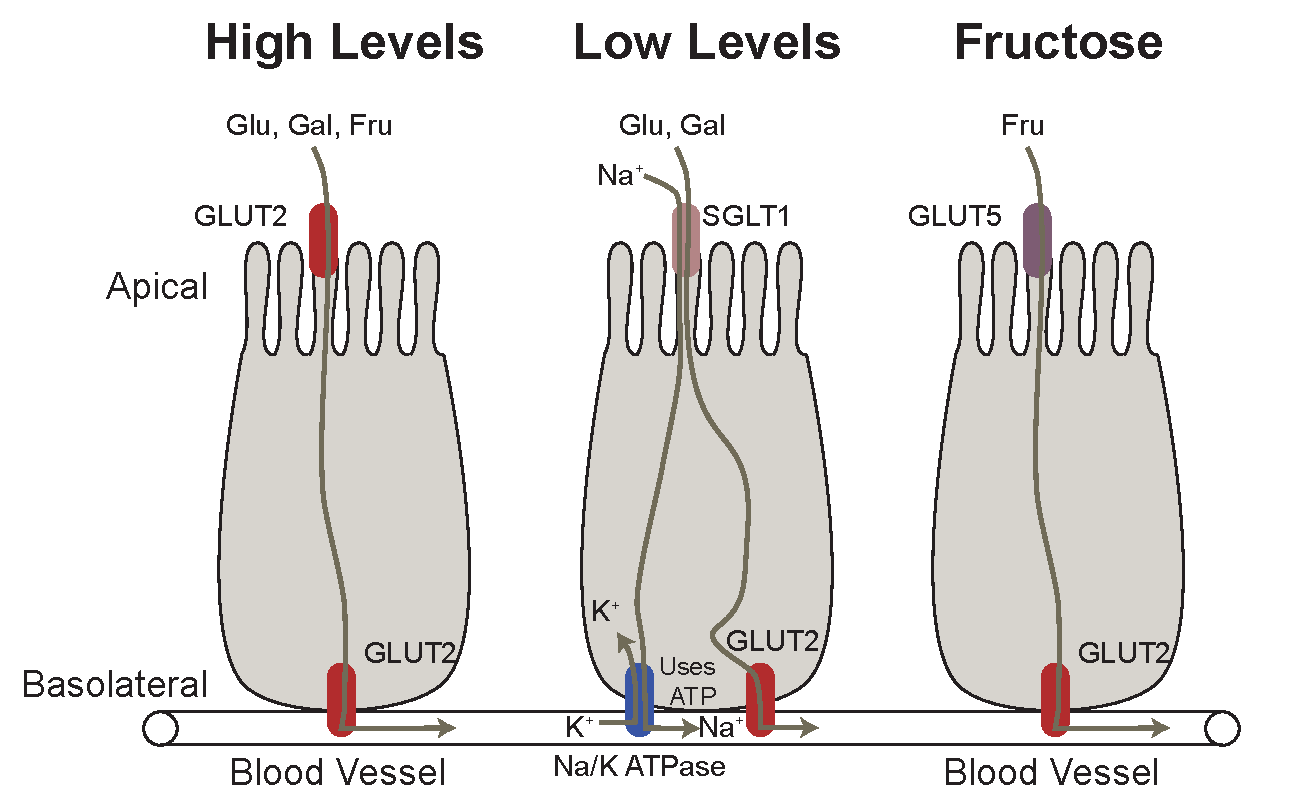
\includegraphics{figures/glucose-intestine.pdf}
\caption{Small intestinal glucose transporters.}
\label{fig:glucose-intestine}
\end{figure}


\subsection{Glucose and Galactose}\index{Carbohydrates!Glucose}\index{Carbohydrates!Galactose}

When glucose and galactose are present in lower concentrations in the lumen in comparison to the enterocyte, they require the SGLT1 transmembrane transport protein to cross the apical membrane. This transport system relies on the high sodium concentration in the lumen.

SGLT1 binds to glucose or galactose and to two sodium ions. Once sodium is bound, this allows for passive diffusion through the apical membrane into the enterocyte. Glucose and galactose are then released and carried through the basolateral membrane via GLUT2\index{Transporters!GLUT2}. To keep the lumen sodium concentrations high and enterocyte sodium concentrations low, the Na/K ATPase pump (energy required) pumps sodium out of the cell and potassium in, thus making this an \emph{active carrier-mediated transport system}
(Figure \ref{fig:glucose-intestine})\emph{.}

\subsection{Fructose}\index{Carbohydrates!Fructose}

Fructose is transported by GLUT5 across the apical membrane and by GLUT 2 across the basolateral membrane.  Recent work has shown that this system is easily saturable \citep{Jang2018}.  At low levels of fructose, it is often converted to glucose and exported to the blood but at higher levels it can enter the circulation as fructose or stay in the gastrointestinal tract resulting in fermentation by the gut microbiota.  That in turn can become acetate and result in hepatic lipogenesis \citep{Zhao2020a}.\index{Gut Microbiome}\index{Lipids!De Novo Lipogenesis}\index{Lipids!Lipid Synthesis}\index{Metabolites!Acetate}\index{Lipids!Fatty Acids!Short Chain Fatty Acids}\index{Non-Alcoholic Fatty Liver Disease}

\newthought{Glucose, Fructose and Galactose -- under conditions of high lumen concentrations}\index{Carbohydrates!Glucose}\index{Carbohydrates!Galactose} \index{Carbohydrates!Fructose}Following high carbohydrate intake, SGLT1 becomes saturated so GLUT2\index{Transporters!GLUT2} is translocated to the apical membrane to assist with transportation across the membrane via passive diffusion \citep{Kellett2008}. Under this mechanism the three monosaccharides will still cross the basolateral membrane via GLUT2. In addition to SGLT1 saturation, the activation of the ``sweet taste'' receptors in the enteroendocrine cells of the digestive tract have been shown to play a role in the translocation of GLUT2 to the apical membrane. This is triggered by monosaccharides as well as sugar substitutes \citep{Stearns2010}. The small intestine is sensitive to insulin, which is released from the pancreas following glucose absorption. The insulin response results in the internalization of GLUT2\index{Transporters!GLUT2} (translocation away from the apical membrane) thus decreasing the absorption rate of glucose. Lastly, mRNA expression of GLUT2 is increased after consumption of a high carbohydrate meal \citep{Miyamoto1993}. This is not unique to GLUT2, but has also been found for GLUT5\index{Transporters!GLUT5} and SGLT1. Thus, there are multiple levels of transporter regulation at the small intestine that influence monosaccharide absorption.
\index{Transporters!SGLT1|)} 


\section{Systemic Carbohydrate Transport}

Once the monosaccharides cross the basolateral membrane, they are small enough molecules that they are able to enter the capillary system eventually entering the hepatic portal vein leading to the liver \index{Liver}\sidenote{hepatic = liver}. Galactose and fructose\index{Carbohydrates!Galactose}\index{Carbohydrates!Fructose} will undergo metabolism in the liver and sm all intestine to be converted into glucose and its derivatives. Glucose can be stored as glycogen\index{Glycogen}, oxidized for energy, broken down for fatty acid or amino acid synthesis or reenter circulation to tissues, all dependent on the body's energy status.

Transportation across cell membranes outside of the intestine requires glucose transporters. As stated earlier, the glucose transporters are
tissue specific thus the isoform present is dependent upon the tissue type (Table \ref{tab:glut-transporters}). Glucose requires insulin signaling to be taken up by GLUT4 at skeletal muscle and adipose tissue.\index{Transporters!GLUT4|(}\index{Muscle}\index{Adipose Tissue}

% Please add the following required packages to your document preamble:
\begin{table}[]
\caption{Summary of major carbohydrate transporters}\index{Transporters!GLUT1}\index{Transporters!GLUT2}\index{Transporters!GLUT5}
\begin{tabular}{llll}\toprule
\label{tab:glut-transporters}
%\toprule
\textbf{Isoform} & \textbf{Expression}              & \textbf{Substrates} \\ \midrule
GLUT1            & CNS, Placenta                    & Glu, Gal             \\
GLUT2            & Liver, Pancreas, Small Intestine & Glu, Gal, Fru        \\
GLUT4            & Adipose, Muscle                  & Glu                    \\
GLUT5            & Small Intestine                  & Fru                 \\ \bottomrule
\end{tabular}

\end{table}


\section{Insulin Resistance and Diabetes}\index{Insulin Resistance|(}

GLUT4\index{Transporters!GLUT4} is a key glucose transporter found on muscle and adipose tissue. This transporter is unique because to function properly it is dependent on proper insulin signaling. Under normal conditions, pancreatic beta-cells\index{Pancreatic beta cells}\index{Pancreas} respond to an increase in blood glucose levels by secreting insulin\index{Hormones!Insulin} into the bloodstream. Insulin receptors are located on skeletal muscle and adipose tissue that bind insulin under these conditions. Once insulin is bound this sends a phosphatidylinositol-3-kinase signal cascade within the cell that releases stored GLUT4 from golgi apparatus in the form of a GLUT4 storage vesicle (GSV). The GSV carries GLUT4 to the cell membrane, releases it and allows for passive diffusion of glucose into the cell.\index{Transporters!GLUT4|)}

\newthought{Insulin insensitivity is a condition that is associated with obesity}\index{Obesity}, Type 2 Diabetes\index{Diabetes, Type 2} and other chronic conditions \citep{DeFronzo2010}. It occurs when the muscle and adipose tissue cells become unresponsive to this insulin signal for cellular glucose uptake resulting in elevated blood glucose levels\index{Blood Glucose Levels}. Because glucose remains in the blood, the pancreas\index{Pancreas} secretes additional insulin to continue to work on getting glucose into cells and also stimulates gluconeogenesis (biosynthesis of glucose by the liver\index{Liver}) because it thinks the cells are deprived of glucose. When this is a continuous occurrence, the pancreatic beta-cells become overworked and stop producing sufficient insulin resulting in long-term hyperglycemia leading to Type 2 Diabetes, heart disease \index{Cardiovascular disease}and other vascular disease. There are several mechanisms that have been hypothesized as playing a role in the mechanism of a cell becoming unresponsive to the insulin signal such as inflammation, genetics and epigenetics. One studied mechanism is \textbf{lipotoxicity}\index{Lipodystrophy} in which excess fat buildup within the body results in fat\index{Adipose Tissue} residing on or within cellular space. This can result in disruption of the insulin pathway by cellular damage and inflammation.
\index{Carbohydrates!Transport|)}\index{Insulin Resistance|)}

\subsection{Glycemic Index} For individuals who suffer from hyperglycemia, diet can play a key role for controlling their blood level of glucose throughout the day.  Carbohydrate-containing food have been categorized by a \textbf{glycemic index}. This index is an indication of the absorption rate of monosaccharides from the small intestine after consuming carbohydrate-containing food \citep{Atkinson2008,Dodd2011}.\index{Glycemic Index}

The index ranges from 1-100 where 100 is the reference of the fastest absorption potential and often symbolized by white bread. As a rule of thumb, foods higher in fiber and lower in fat have a lower glycemic index and more processed foods (decreased fiber content) have a higher glycemic index (Table \ref{tab:glycemic index}). The glycemic index is a tool that can be used to help educate individuals on proper food choices to help control flux of carbohydrate absorption and to help maintain a steady level of blood glucose when consuming food and throughout the day.

% Please add the following required packages to your document preamble:
% \usepackage{booktabs}
\begin{table}[b]
\caption{Examples of foods by glycemic index}
\label{tab:glycemic index}
\begin{tabular}{{p{3cm}p{7cm}}}
\toprule
\textbf{Glycemic Index} & \textbf{Example Foods} \\ \midrule
\textless{}55 Low & Steel cut oatmeal, fruits, whole wheat bread, corn tortillas, tomato juice \\
55-69 Medium & Quick oats, brown rice, rye bread, bagels, fruit juices \\
69-100 High & White bread, instant oatmeal, white rice, popcorn, soda \\\bottomrule
\end{tabular}
\end{table}

\section{Lactase Non-persistence}\index{Lactase Non-Persistence |(}\index{Digestive Enzymes!Lactase|(}\index{Carbohydrates!Lactose|(}

\newthought{Lactose intolerance} is a common term used to describe the overarching symptom of the condition of \textbf{lactase non-persistence}. This condition results from an enzyme deficiency of the digestive enzyme lactase, described above. In mammals, the lactase gene\sidenote{The gene symbol is \textit{LCT}} is highly active in the lactation life stage (\textit{i.e.}, infancy) when the sole food intake is from the mother's lactose-containing breast milk\index{Breast milk}. Following the introduction to other food products, and consequently, exposure to foods containing carbohydrates other than lactose, the production of lactase rapidly declines, as there is no significant need for its activity.

Because of the innovation of domesticating milk-producing animals, humans are a unique mammal because this allows us the opportunity to
continue to drink milk and eat milk-based food products beyond the lactation period \citep{Itan2009}. Over time some humans developed a genetic polymorphism\index{Genetic variation} in the lactase gene resulting in sufficient production of lactase throughout adulthood when there is continuous exposure to lactose-containing foods. Because milk-producing agriculture is a recent event in regard to evolution this polymorphism is thought to arise from a high frequency haplotype due to the benefit of ingesting lactose in cultures that raise milk-producing animals \citep{Harvey1998,Itan2009}. Individuals lacking this polymorphism will have a decline in lactase production and will start to have symptoms of lactose intolerance in early childhood.

Specific symptoms include bloating, cramping and diarrhea\index{Diarrhea}. Because the disaccharide lactose will not be properly digested for absorption, it will travel to the large intestine \index{Large Intestine} where it can absorb and retain water within the large intestine causing bloating and potentially diarrhea and dehydration. Of note, it has been evidenced that individuals who are \textbf{lactase persistence} but do not expose themselves to milk-containing products will have a steady decline of lactase production over time and may also exhibit symptoms of
lactose intolerance when reintroducing milk-products \citep{Gerbault2011}.
\index{Lactase Non-Persistence |)}\index{Digestive Enzymes!Lactase|)}\index{Carbohydrates!Lactose|)}


\bibliography{library}
\bibliographystyle{plainnat}
\end{document}
